% Revised 2026-09-28 after the second technical review; source audit targets revision 4b5dab4.
% Self-contained: vector figures and references are embedded.
% Author metadata is awaiting the owner's supplied details.
\documentclass[conference,a4paper]{IEEEtran}
\usepackage[T5,T1]{fontenc}
\usepackage[utf8]{inputenc}
\usepackage{amsmath,amssymb,booktabs,array,tabularx}
\usepackage{cite,url,graphicx,xcolor,tikz}
\usetikzlibrary{arrows.meta,positioning,calc,fit}
\usepackage[hidelinks]{hyperref}
\newcommand{\viet}[1]{{\fontencoding{T5}\fontfamily{ptm}\selectfont #1}}
\newcommand{\sys}{S_{\mathrm{hybrid}}}
\newcommand{\code}[1]{\texttt{#1}}
\definecolor{ink}{HTML}{18324D}
\definecolor{bluewash}{HTML}{EDF4FB}
\definecolor{greenwash}{HTML}{EBF5F0}
\definecolor{amberwash}{HTML}{FFF5E6}
\definecolor{linegray}{HTML}{526477}
\tikzset{
box/.style={draw=linegray,rounded corners=2pt,line width=.5pt,fill=bluewash,align=center,inner sep=4pt,font=\sffamily\footnotesize,text=ink},
step/.style={box,text width=6.6cm,minimum height=.58cm},
narrow/.style={box,text width=3.05cm,minimum height=.65cm},
arr/.style={-{Stealth[length=1.6mm]},line width=.65pt,draw=linegray},
note/.style={font=\sffamily\scriptsize,align=center,text=ink,fill=white,inner sep=1.2pt}}
\setlength{\emergencystretch}{1.5em}
\raggedbottom
\title{SalePilot: Inspectable Constraint-Aware Recommendation\\for Vietnamese Retail Consultation}
\author{}
\begin{document}
\maketitle

\begin{abstract}
Vietnamese retail consultation requires a system to interpret informal requests, retain needs across turns, and check product constraints before offering alternatives. SalePilot combines a deterministic recommender with optional large language model orchestration in a web application. We describe the current implementation, including state persistence, admission rules, score terms, and decision fingerprints. An author-side audit of archived scores covers 40 developer-authored, single-turn episodes. Across all scored payloads, including clarification payloads, the rows record 10 violations in 117 product--constraint checks for a price--popularity baseline and none in 99 checks for either constraint-aware policy. Recommendation-action coverage is 80\% versus 70\%. On 28 common recommendation episodes, counts are 7/99 versus 0/99. These are descriptive historical observations: original predictions and the evaluation catalog are missing, and the historical run's code and configuration versions are not recorded. The paper-only supplement supplies a derived report, not the raw inputs needed to repeat that audit. The contribution is an implementation specification with exploratory evidence, without establishing causal filtering effects, ranking superiority, or current end-to-end performance.
\end{abstract}
\begin{IEEEkeywords}
conversational recommendation, Vietnamese retail, constraint checking, decision evidence, evaluation audit
\end{IEEEkeywords}

\section{Introduction}
Conversational recommenders gather requirements through interaction rather than treating every request as a complete query~\cite{jannach2021survey}. In retail, a wrong width or budget can make an otherwise attractive product unusable. A useful system must also decide when the available information is insufficient.

Question selection and the separation of preference estimation from action choice are established themes in conversational recommendation~\cite{christakopoulou2016towards,lei2020ear}. SalePilot implements these concerns as inspectable rules for Vietnamese appliance and electronics requests. Product facts come from a normalized catalog; optional language models coordinate tools and formulate responses.

The technical question is how to expose the relationship between a parsed need, admission decisions, a ranked list, and its underlying data. A second question is what a small offline comparison can establish when policies recommend at different rates and its historical provenance is incomplete.

This paper contributes (i) a source-grounded account of the current web runtime and state persistence; (ii) an explicit description of its scoring, comparison policies and fingerprint semantics; and (iii) an author-side audit of archived evaluation rows, including action coverage and a common-episode comparison. The implementation account targets revision \code{4b5dab4}, inspected on 28 September 2026, in \url{https://github.com/VanAnh-13/SalePilot_Agent}. The full commit and inspected-file hashes are in the supplement. Archived measurements are not presented as a rerun of that revision, and the paper-only package does not contain application source or raw audit inputs.

\section{Related Work}
Conversational recommendation combines language understanding, dialogue management, and recommendation~\cite{jannach2021survey}. EAR separates estimation, action, and reflection~\cite{lei2020ear}. SalePilot uses a rule-based need state and action logic; it does not reproduce EAR's learned policy.

ReAct alternates language-model reasoning and tool actions~\cite{yao2023react}. Hybrid agents have also been studied for e-commerce recommendation~\cite{nie2024hybrid}. SalePilot's Lead--tools loop follows this general organization, while clear recommendation requests can bypass the graph.

Component scores and users' experience measure different aspects of conversational systems~\cite{jannach2023evaluating}. Reproducibility work motivates explicit baselines and complete experimental records~\cite{ferraridacrema2021troubling,pineau2021reproducibility}. We distinguish source inspection, reaggregation of stored scores, and executable reproduction. A decision payload supports inspection of product facts; it does not establish faithful interpretation of a language model's internal reasoning~\cite{jacovi2020faithfulness}.

\section{Current Implementation}
\subsection{Architecture and request routing}
The supported customer-facing channel is the web interface. Next.js calls FastAPI's \code{/chat} or \code{/chat/stream}. The server derives the conversation from the web channel and external identity, stores messages, and checks for human takeover. The client identity is not an authenticated account.

\begin{figure*}[t]
\centering
% FIGURE: current_architecture
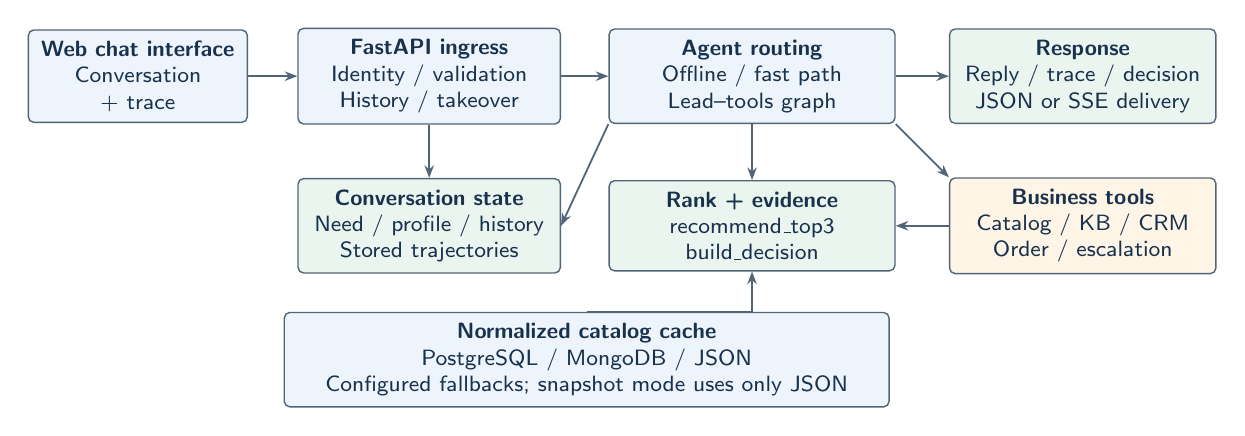
\begin{tikzpicture}
\node[box,text width=2.5cm,minimum height=.9cm] (web) at (0,0) {\textbf{Web chat interface}\\Conversation + trace};
\node[box,text width=3.05cm,minimum height=.9cm] (api) at (3.7,0) {\textbf{FastAPI ingress}\\Identity / validation\\History / takeover};
\node[box,text width=3.35cm,minimum height=.9cm] (routes) at (7.8,0) {\textbf{Agent routing}\\Offline / fast path\\Lead--tools graph};
\node[box,text width=3.1cm,minimum height=.9cm,fill=greenwash] (response) at (12,0) {\textbf{Response}\\Reply / trace / decision\\JSON or SSE delivery};
\node[box,text width=3.05cm,minimum height=.85cm,fill=greenwash] (state) at (3.7,-1.9) {\textbf{Conversation state}\\Need / profile / history\\Stored trajectories};
\node[box,text width=3.35cm,minimum height=.85cm,fill=greenwash] (consult) at (7.8,-1.9) {\textbf{Rank + evidence}\\recommend\_top3\\build\_decision};
\node[box,text width=3.1cm,minimum height=.85cm,fill=amberwash] (business) at (12,-1.9) {\textbf{Business tools}\\Catalog / KB / CRM\\Order / escalation};
\node[box,text width=7.4cm,minimum height=.55cm] (catalog) at (5.7,-3.6) {\textbf{Normalized catalog cache}\\PostgreSQL / MongoDB / JSON\\Configured fallbacks; snapshot mode uses only JSON};
\draw[arr] (web)--(api);
\draw[arr] (api)--(routes);
\draw[arr] (routes)--(response);
\draw[arr] (api)--(state);
\draw[arr] (routes)--(consult);
\draw[arr] (routes.south east)--(business.north west);
\draw[arr] (routes.south west)--(state.east);
\draw[arr] (catalog.north)-|(consult.south);
\draw[arr] (business.west)--(consult.east);
\end{tikzpicture}
\caption{Current chat-path architecture. Automated serving routes can persist conversation need and trajectories; the shared consultation function only ranks and builds evidence. The catalog recommendation tool calls the same ranker and decision builder separately; the other business tools do not. Business tools are available directly to the Lead and through role-scoped delegation. The owner dashboard reads separate admin endpoints (not shown). Other responses may have no decision payload.}
\label{fig:architecture}
\end{figure*}

Fig.~\ref{fig:request} shows the actual route order. Without an LLM key, a rule-based coordinator handles recommendation, comparison, FAQ, CRM, and escalation. With a key, the system first tries a deterministic fast path. Missing slots can produce clarification directly. Comparison, policy, contact, and escalation intents normally fall through to the graph; no-match and fast-path failures also fall through.

\begin{figure}[t]
\centering
% FIGURE: current_request_flow
\begin{tikzpicture}[node distance=3.5mm]
\node[step] (ingress) {Web request $\rightarrow$ validate and store user message};
\node[step,below=of ingress] (takeover) {Human takeover active?};
\node[narrow,fill=amberwash,below left=7mm and -3.1cm of takeover] (human) {Yes: save handoff reply\\Skip automated agent};
\node[narrow,below right=7mm and -3.1cm of takeover] (key) {No: load memory\\Is an LLM key configured?};
\node[narrow,below=7mm of human,fill=greenwash] (offline) {No key: offline coordinator\\Shared consultation + intent tools};
\node[narrow,below=7mm of key] (fast) {Key present: try fast path\\Clarify or recommend if handled};
\node[narrow,below=7mm of fast,fill=amberwash] (lead) {Unhandled / no match / error\\Lead $\leftrightarrow$ tools / delegates};
\node[narrow,below=7mm of offline,fill=greenwash] (finish) {Deliver JSON or SSE events\\Assistant persistence varies\\By route and outcome};
\draw[arr] (ingress)--(takeover);
\draw[arr] (takeover.south)-|(human.north);
\draw[arr] (takeover.south)-|(key.north);
\draw[arr] (key.west)--++(-.28,0)|-(offline.east);
\draw[arr] (key)--(fast);
\draw[arr] (fast)--(lead);
\draw[arr] (fast.west)--++(-.2,0)|-(finish.east);
\draw[arr] (lead.west)--++(-.22,0)|-(finish.south east);
\draw[arr] (offline)--(finish);
\draw[arr] (human.west)--++(-.22,0)|-(finish.west);
\end{tikzpicture}
\caption{Request control flow. An ordinary batch reply is saved with trace metadata before JSON return. On automated streaming routes, events (including \code{done}) precede saving a nonempty assistant reply; a terminal stream error can leave no assistant save. Human takeover saves an acknowledgment with a takeover flag before delivery and creates no agent trajectory. The Lead finishes via \code{finalize} or final text. Caught graph-execution errors use a fallback only if no final reply exists; other stream failures emit an error event. An empty deterministic list is not a universal runtime abstention.}
\label{fig:request}
\end{figure}

The LangGraph graph alternates between the Lead and the ToolNode. The Lead can call business tools directly or use \code{delegate}/\code{delegate\_many}; specialist roles are catalog, knowledge, CRM, order, and escalation. Each specialist receives a tool allowlist. The graph stops on a final response or a configured limit.

Fast-path LLM phrasing is optional and disabled by default; its timeout or failure falls back to deterministic formatting. The graph route can stream Lead text, whereas deterministic routes emit a completed result as batched events. Neither streaming nor language quality is evaluated by the archived benchmark.

\subsection{Need state, category scope, and clarification}
Let $u_t$ be the current user text, $n_{t-1}$ the stored need, and $p_t$ the available customer profile. First define $h_t$ as the working prior state. On the offline route only, if the stored category is explicitly negated in $u_t$, retain only its budget and brand in $h_t$ and save that reduced state immediately. Otherwise $h_t=n_{t-1}$. Let $D$ detect a category, with $\bot$ meaning none. The category context and initial merge are
\begin{align}
d_t&=D(u_t),\quad c_t=\begin{cases}d_t,&d_t\ne\bot,\\h_t[\mathrm{category}],&d_t=\bot,\end{cases}\label{eq:context}\\
m_t&=M\!\left(h_t,E(u_t,c_t)\right).\label{eq:state}
\end{align}
An absent stored category is also $\bot$. Here $E$ normalizes configured Vietnamese abbreviations and extracts budget, brand, category slots, and priorities. $M$ overwrites fields with fresh nonempty values and unions priorities within one category.

On a category switch, $M$ discards previous category fields, priorities, and stored product choices. It retains the old budget if no new budget is extracted. This is a conversation-wide budget heuristic in the current code, without confirmation for the new category.

Let $s_t$ mean that both a fresh and a stored category exist and differ, using $h_t$ as the prior state. Let $F(m,h,u)$ be the follow-up resolver and $P(z,p)$ fill budget from the profile only when absent in $z$ and nonzero in $p$. The post-merge need is
\[
z_t=\begin{cases}m_t,&s_t,\\F(m_t,h_t,u_t),&\text{otherwise},\end{cases}
\qquad q_t=P(z_t,p_t).
\]
Both deterministic runtime routes use this order. $F$ checks slots pending in $h_t$: a bare number first fills an unfilled product slot, multiplied by its configured unit factor; otherwise $0<a\le500$ fills a pending budget as $a$ million VND. Recognized room labels fill an unfilled area slot using approximate areas. Existing fresh values take precedence.

Persistence is conditional. Let $G_t$ mean that a category is present and the route enters product consultation: the fast path's recommendation-intent check passes, or the offline routing policy sets \code{need\_product}. Let $\Pi$ remove \code{raw} and entries equal to null, empty string or empty list, matching \code{save\_need}. With memory enabled and a nonempty external identity, on normal completion of this deterministic stage the next stored need is
\[
n_t=\begin{cases}
\Pi(L(q_t,T_t)),&G_t,\\
h_t,&\text{otherwise},
\end{cases}
\]
where $T_t$ is the returned list and $L$ adds its nonempty SKU list as \code{last\_skus}, leaving $q_t$ unchanged for an empty list. Each save applies $\Pi$, including the offline negation save. If memory is disabled or the identity is empty, saves are no-ops. The routes save $q_t$ around consultation and save again when SKUs are available. Thus clarification stores the projection of the post-resolution, post-profile need, before any ranker-local removal of an irrelevant household slot. No-match on the fast path can save this need before falling through to the graph. This transition specifies the deterministic stage; later graph tools and exceptional partial writes are outside its scope.

\begin{figure}[t]
\centering
% FIGURE: current_need_flow
\begin{tikzpicture}[node distance=3mm]
\node[step] (detect) {Current text + stored need\\Offline only: clear and save negated category first\\Detect fresh category; otherwise use working prior};
\node[step,below=of detect] (merge) {Extract and merge\\Same category: overwrite fields, union priorities\\Switch: reset category fields; keep old budget if not replaced};
\node[step,below=of merge,fill=greenwash] (resolve) {Runtime follow-up resolution\\Skip on switch; otherwise resolve number / room label\\Fill absent budget from profile};
\node[step,below=of resolve] (gate) {Shared consult: check category and required slots\\Apply force bypass only for a recognized category};
\node[narrow,below left=6mm and -3.05cm of gate,fill=amberwash] (ask) {Missing: clarification + decision\\Save need if route permits\\Wait for next user turn};
\node[narrow,below right=6mm and -3.05cm of gate,fill=greenwash] (rank) {Ready: rank + decision\\Persist need on eligible route\\Store SKUs if list nonempty};
\draw[arr] (detect)--(merge);
\draw[arr] (merge)--(resolve);
\draw[arr] (resolve)--(gate);
\draw[arr] (gate.south)-|(ask.north);
\draw[arr] (gate.south)-|(rank.north);
\draw[arr] (ask.west)--++(-.2,0)|-(detect.west);
\end{tikzpicture}
\caption{Need update on deterministic product-consultation routes; persistence is conditional on $G_t$ and may occur before or after consultation, depending on the route. The experiment adapter omits profile filling and follow-up resolution. Its 40 test episodes each contain one user turn.}
\label{fig:need}
\end{figure}

The recommender asks for a budget unless flexibility is explicit. If a category has a primary sizing slot, supplying any configured category slot satisfies the current sizing gate. This does not guarantee the primary slot itself is present. For a recognized category, \code{force} bypasses budget and product-slot questions; the tool helper also sets budget flexibility when forced. An unknown category still triggers clarification.

The crawl registry defines detailed rules for eight families and adds generic objects for other loaded categories. Generic categories have aliases and budget-oriented ranking without detailed slots. The separate engineering workbook registry contains 14 categories.

\subsection{Admission and scoring}
For a need $n$, the ranker selects category records with a price. Admission is implemented inside \code{\_score}, using a rejection sentinel. Nonflexible over-budget items are rejected. Known minimum/maximum violations are rejected; hard range violations and missing hard facts are rejected according to slot policy.

For an admitted product $p$, the implemented score is
\begin{equation}
\begin{split}
S(p,n)={}&B(p,n)+3I_b+4I_s\\
&+\sum_{k\in K(n)} f_k(p,n)+\sum_{j\in J(n)}g_j(p,n)+Q(p).
\end{split}\label{eq:score}
\end{equation}
$K(n)$ contains supplied category slots and $J(n)$ the recognized priorities. $I_b$ indicates a matching preferred brand, and $I_s$ a matching explicitly supplied style. These indicators are zero when the corresponding preference is absent. Scores are dimensionless heuristic points; coefficients are configured, not learned.

For finite inputs in the intended nonnegative domain, let $v\in\mathbb{Z}_{\ge0}$ be price and $b\in\mathbb{Z}_{\ge0}\cup\{\bot\}$ be budget, both in VND. This domain is an assumption for the equations, not an enforced invariant: the crawl price parser accepts negative numeric values and the ranker only checks whether price is present. Only when $b\ne\bot$, define $\bar b=\max(b,1\,\mathrm{VND})$. The budget contribution on admitted products is
\begin{equation}
B=\begin{cases}
0,&b=\bot,\\
4+\max(0,\,2-2(b-v)/\bar b),&b\ne\bot,\ v\le b,\\
-\min(6,\,10(v-b)/\bar b),&b\ne\bot,\ v>b,\ \text{flexible}.
\end{cases}\label{eq:budget}
\end{equation}
The remaining case, $v>b$ without flexibility, is inadmissible. Flexibility therefore permits an over-budget recommendation with a penalty.

Table~\ref{tab:slots} defines $f_k$. $w$ is the slot weight, $x$ a normalized product fact, and $q$ the requested value in the same configured unit. The denominator $\max(q,1)$ uses a one-unit floor in that unit; it is not invariant to an arbitrary change of units.

\begin{table}[t]
\caption{Slot contributions and admission behavior}
\label{tab:slots}
\centering\footnotesize
\begin{tabularx}{\columnwidth}{@{}p{1.35cm}X@{}}
\toprule
Slot kind & Implemented behavior\\
\midrule
Range fit & Inside known bounds: $+w$. Outside: reject if hard; otherwise $-(w+2)$. A missing endpoint leaves that side unbounded. Both absent: reject if hard and policy is not \code{allow\_unknown}; otherwise $-w/2$.\\
Maximum / minimum & Known fact violates bound: reject. Satisfied bound: $+1$. Missing fact: reject only for hard + \code{exclude}; otherwise $-w/2$.\\
Proximity & Known fact: $\max[-0.6w,\ w-w|x-q|/\max(q,1)]$. Missing fact: $-0.4w$.\\
\bottomrule
\end{tabularx}
\end{table}

For numeric priorities, extrema $\ell_j,h_j$ are computed over all priced category products before admission, using available convertible values. Let $x_j$ be the product's corresponding price or specification and $a_j$ its configured direction. Define the contribution directly, so the ratio is evaluated only on a nondegenerate range:
\[
g_j=\begin{cases}
0,&x_j=\bot\ \text{or}\ h_j\le\ell_j,\\
w_j\dfrac{x_j-\ell_j}{h_j-\ell_j},&x_j\ne\bot,\ h_j>\ell_j,\ a_j=\mathrm{max},\\
w_j\left(1-\dfrac{x_j-\ell_j}{h_j-\ell_j}\right),&x_j\ne\bot,\ h_j>\ell_j,\ a_j=\mathrm{min}.
\end{cases}
\]
Cheap-price and minimum-specification preferences use $a_j=\mathrm{min}$. Missing extrema use $(0,0)$ and therefore contribute zero.

Boolean/presence priorities contribute $w_j$ for a nonempty, nonzero value and $-w_j/2$ otherwise. Text priorities contribute $w_j$ on a configured substring match and $-1$ otherwise. On normalized data, rating $\rho\in\mathbb{R}_{\ge0}\cup\{\bot\}$ and sold count $s\in\mathbb{Z}_{>0}\cup\{\bot\}$. Their secondary contributions are
\[
Q_\rho=\begin{cases}0,&\rho\in\{\bot,0\},\\0.6(\rho-4),&\rho>0,\end{cases}\quad
Q_s=\begin{cases}0,&s=\bot,\\\min(1,\log_{10}(s+1)/5),&s>0.\end{cases}
\]
The crawl importer maps an unparseable or nonpositive rating to missing and rounds positive ratings to one decimal; a small positive value can round to zero, and there is no clamp at five stars. It parses a leading sold-count number with optional thousand/million suffix, rounds to an integer and maps zero or unparseable text to missing. The ranker also skips numeric zero. These are ingestion conventions, not runtime validation guarantees: direct database/snapshot values are not re-sanitized, and malformed or negative counts may cause conversion or logarithm errors. The equations assume finite normalized values. $Q$ additionally adds $0.5$ when both nonzero prices indicate a sale and $0.3$ for a nonempty gift promotion.

\begin{figure}[t]
\centering
% FIGURE: current_ranking_flow
\begin{tikzpicture}[node distance=3mm]
\node[step] (input) {Need + category registry + normalized catalog};
\node[step,below=of input] (gate) {Unknown category or required information missing?\\Return clarification + decision; otherwise continue\\Force can bypass budget / product-slot questions};
\node[step,below=of gate] (score) {Priced category candidates\\Compute ranges; admission checks inside scoring\\Reject sentinel or score from Eq.~(\ref{eq:score})};
\node[step,below=of score,fill=greenwash] (sort) {Sort: score descending, price ascending\\Exact ties preserve repository input order};
\node[step,below=of sort,fill=greenwash] (select) {Deduplicate by model code (fallback SKU)\\Prefer distinct brands while selecting first two\\Fill remaining positions up to three};
\node[step,below=of select,fill=amberwash] (decision) {One-pass decision payload\\Need / selected facts / statuses / counts / hashes\\No candidate: empty result, handled by serving route};
\draw[arr] (input)--(gate);
\draw[arr] (gate)--(score);
\draw[arr] (score)--(sort);
\draw[arr] (sort)--(select);
\draw[arr] (select)--(decision);
\end{tikzpicture}
\caption{Conceptual ranking stages corresponding to current code. Clarification exits before scoring. Equal score/price ties have no SKU tiebreaker, so backend-independent ordering is not guaranteed.}
\label{fig:ranking}
\end{figure}

Equal score/price ties retain input order. The selector deduplicates exact model codes (falling back to SKU), prefers distinct brands while choosing the first two items, and fills up to three positions. This is not similarity-based duplicate detection; brand-diversity choices can depart from simple score order.

\subsection{Decision evidence and its limits}
The shared \code{consult} function ranks once and constructs \code{salepilot-decision-v1} from that result. It records semantic need fields, selected facts, constraint states, candidate and rejection counts when scoring occurred, provenance, a catalog-projection fingerprint, and a decision hash.

States are \code{matched}, \code{violated}, and \code{unknown}. For configured hard slots with an \code{exclude} policy, a missing fact is rendered as violated. A present proximity fact is labeled matched without a separate distance threshold. Budget evidence remains labeled hard even when the ranker accepts an over-budget item under flexibility. These details limit a literal safety interpretation of the status strings.

Exported score components are a budget-fit summary, total match score, and rating where available. They do not enumerate all addends of Eq.~\eqref{eq:score}.

The runtime field named \code{catalog\_hash} is a SHA-256 fingerprint of a field projection over \emph{every loaded catalog record}, not only recommended products. Records are sorted by string SKU then integer category code, defaulting missing/empty values in that sort key to empty string and zero. Each projected object omits fields equal to null, empty string or empty object, then uses Python JSON with sorted keys, compact separators, unescaped Unicode and nonfinite numbers forbidden. UTF-8 bytes of each object, followed by one newline byte, feed SHA-256. Numeric types are not further canonicalized: integer 1 and float 1.0 serialize differently; duplicate sort keys preserve input order.

The projection includes SKU, model code, web product ID, category code/slug/display, brand, name, description, original/sale/current price, current-price flag, gift promotion, outstanding features, rating, sold count, warranty, accessories, color, image URL, product URL, online-only flag, normalized facts (\code{norm}), specifications (\code{specs}), and source row. It omits other fields, including \code{search\_text}, used by $B_1$. Thus identical fingerprints do not prove equality of every ranking input. The payload also supplies loaded-record count and backend label. It has no guaranteed full-snapshot file digest or snapshot locator.

The decision hash uses the same JSON options on the assembled decision without its own hash. Its hash input retains only catalog hash/count in the top-level source object and removes each item's provenance backend label; item order and remaining provenance still matter. A separate experiment-runner pin hashes the complete snapshot file bytes and records its path. That pin, the projection fingerprint and the decision hash are distinct objects. A digest supports content comparison, not factual correctness or recovery of missing data.

The repository supports PostgreSQL, MongoDB, and JSON. Database modes use configured fallback order; snapshot mode uses only the snapshot. Identical normalized content does not guarantee identical lists because ranking ties depend on input order.

\section{Data and Evaluation Materials}
\subsection{Available catalog and policy summaries}
The stored catalog summary inspected in the full repository describes 13{,}754 products in 119 categories and 436 brands; 13{,}739 products have prices. Its reported price range is 10{,}000--380{,}000{,}000 VND, with median 1.39 million VND and mean approximately 6.14 million VND. These are stored aggregates, not a fresh census of a running database. The paper-only supplement reproduces them in its derived report.

The largest category contains 3{,}138 products (22.8\%). The top 15 categories contain 9{,}188 products; the remaining 104 contain 4{,}566 (33.2\%). This imbalance motivates generic category support but does not imply equal quality across categories. The available specification index has 1{,}348 keys; the policy FAQ file contains 106 chunks.

The tool-schema summary records 56 calls across seven tools: order creation 22, product search 17, delivery-time queries 11, customer-information checks 3, and comparison, payment, and installment links one each. Order creation and search account for 39/56 (69.6\%). These aggregates do not measure SalePilot conversion. Unreconciled message-role totals and unverifiable field-coverage and price-bin statistics are not used as quantitative evidence.

\subsection{Archived benchmark and boundary}
The benchmark has 40 developer-authored test episodes, each with one user turn. Gold actions are 32 \code{recommend}, one \code{clarify}, two \code{faq}, and five \code{abstain}. The schema permits \code{compare}, but the test split has no examples. There are 11 non-null labeled product categories.

The historical manifest names a 13{,}716-product, 118-category catalog. That snapshot is absent from this checkout. Its relationship to the larger stored catalog summary cannot be reconstructed from counts alone.

The adapters share category detection, extraction, and merge functions, then score the final user turn. They bypass the Web gateway, persistent memory, runtime follow-up resolver, Lead graph, specialist loops, and response generation. They do not evaluate the current multi-turn runtime.

Table~\ref{tab:policies} specifies the currently inspected adapters. All start with an empty need and, for each user turn, extract without stored-category context and merge; $B_1$ then removes both priority fields. No adapter calls the runtime follow-up resolver or loads a profile. These code definitions explain possible action/payload combinations, but the absent generating revision prevents certifying that every historical prediction used precisely this implementation. The optional LLM comparator is excluded because its historical provider and prediction records do not form a consistent experimental chain.

\begin{table*}[t]
\caption{Current adapter definitions; historical generating code is not pinned}
\label{tab:policies}
\centering\footnotesize
\begin{tabularx}{\textwidth}{@{}p{1.8cm}XXX@{}}
\toprule
Stage & $B_0$: price/popularity & $B_1$: lexical/filter & $\sys$: production ranker\\
\midrule
Information gate & \code{need\_more} if category or budget is absent/zero, but candidates are still constructed. Ignores sizing, force and budget flexibility. & Unknown category or \code{pending\_slots} yields clarification and no candidates; no force bypass. & Unknown category always clarifies. Required slots gate ranking, unless force is set for a known category.\\
Admission & Category records with a price; enforce any parsed budget even if flexible. No slot admission rules. & Category records passing budget and slot rules below. No price-presence gate when budget is absent. & Priced category records; budget and slot branches in Section III-C.\\
Score and order & Sold count descending, price ascending; missing sold becomes zero. & Unit-weight lexical hits descending, sold descending, price ascending, then SKU string ascending. & Eq.~\eqref{eq:score} descending, price ascending.\\
Selection & First three; no model deduplication or brand diversification. & First three; no model deduplication or brand diversification. & Model deduplication and brand-diverse selection, up to three.\\
Empty result & \code{ok=false}; missing-information flag may still be true. & If gate passed, \code{ok=false}, \code{need\_more=false}. & If gate passed, \code{ok=false}, \code{need\_more=false}.\\
\bottomrule
\end{tabularx}
\end{table*}

For $B_1$, tokens are unique Unicode word tokens from case-folded final user text, of length at least three, excluding \viet{cần}, can, mua, \viet{dưới}, duoi, \viet{triệu}, trieu, \viet{khoảng}, and tam. Its score counts one point for each token occurring as a substring in case-folded \code{search\_text}, falling back to product name. It has no learned weights. Price sort keys use $10^{15}$ VND for missing or zero price; $B_0$ and the hybrid use the same zero-price fallback. Fully equal keys retain input order.

$B_1$ rejects missing/over-budget prices when a budget exists, even if flexible. For a supplied range-fit slot, a hard constraint rejects out-of-range values or two missing endpoints regardless of the slot's missing policy; a single missing endpoint is unbounded. Soft range-fit slots impose no filter. Known maximum/minimum violations reject; missing facts reject only when hard and policy differs from \code{allow\_unknown}. Proximity slots do not filter or score. Its information gate uses the budget/primary-slot rules described in Section III-B; unlike the hybrid, it never applies force bypass.

All three construct a result and decision before the same ordered action inference: (1) unsupported-category detection gives abstain; (2) a literal case-folded substring among \viet{còn hàng}, \viet{tồn kho}, \viet{bảo hành}, and \viet{giao hàng} gives FAQ; (3) \code{need\_more} gives clarify; (4) \code{ok} plus nonempty \code{top3} gives recommend; (5) otherwise abstain. There is no comparison action. The action mapper does not clear products already in the payload. In particular, $B_0$ can return products with a missing-budget flag and therefore predict clarification. With gate-passing empty results, the last branch gives abstain unless an earlier text rule takes precedence.

\begin{figure}[t]
\centering
% FIGURE: current_evaluation_flow
\begin{tikzpicture}[node distance=3mm]
\node[step] (labels) {Author-side inputs: 40 labels + 120 score rows\\Paper-only package: derived audit report\\Gold R=32, C=1, F=2, A=5; compare=0};
\node[step,below=of labels,fill=amberwash] (audit) {Check provenance before interpreting results\\Label hashes match; score hash matches with CRLF\\Original predictions, historical catalog, bootstrap files absent};
\node[step,below=of audit] (group) {Reaggregate archived rows by condition\\$B_0$: popularity / $B_1$: lexical filter / $\sys$};
\node[step,below=of group,fill=greenwash] (measure) {Action accuracy + confusion + recommendation coverage\\All payload checks; recommendation-only sensitivity\\Common recommendation episodes};
\node[step,below=of measure,fill=amberwash] (interpret) {Descriptive evidence only\\No current prediction rerun, causal attribution,\\ranking-utility claim, or independent reproduction};
\draw[arr] (labels)--(audit);
\draw[arr] (audit)--(group);
\draw[arr] (group)--(measure);
\draw[arr] (measure)--(interpret);
\end{tikzpicture}
\caption{Author-side analysis in the full repository. The paper-only supplement lacks raw inputs and supports report-level arithmetic inspection only. R/C/F/A denote recommend, clarify, FAQ, and abstain.}
\label{fig:evaluation}
\end{figure}

\subsection{Metrics and provenance}
Action and category accuracy use all 40 labels, including null categories. Slot micro-F1 pools slot true positives, false positives, and false negatives. The archived evaluator counts product--constraint pairs from returned \code{top3} payloads regardless of predicted action, applying gold constraints rather than model-generated status labels. An unavailable hard fact counts as a violation unless its gold policy is \code{allow\_unknown}.

Within one fixed policy condition, let $v_e$ and $c_e$ denote recorded violations and checks for episode $e$. For a specified set $A$, the pooled rate is
\begin{equation}
V(A)=\frac{\sum_{e\in A}v_e}{\sum_{e\in A}c_e}.\label{eq:metric}
\end{equation}
The mathematical rate is undefined when the denominator is zero; the evaluator stores \code{0.0} as a sentinel for those cases. Such rows contribute no checks to the pooled ratio. Recommendation-action coverage is the fraction of all 40 episodes predicting \code{recommend}, distinct from products in a payload.

In the inspected repository, the development and test label files match the SHA-256 digests in \code{SEAL\_RECORD.json}. The archived score file, \code{exp\_test\_scores.json}, uses LF line endings; converting only those line endings to CRLF reproduces the digest in \code{CHAIN\_OF\_CUSTODY.json}. The difference in raw file hashes is therefore explained by line-ending representation. The original prediction file and both bootstrap files referenced by that record are absent from this checkout. The record also lacks the code revision and configuration hash for the historical deterministic run. The audit records hashes of the currently inspected code and configuration, but these do not establish which versions generated the archived results. These missing artifacts and version records prevent a complete reconstruction of that run.

We recomputed arithmetic from rows available in the full repository and preserved these provenance limits. The paper-only supplement contains the resulting audit report and script, but not the labels, score rows, manifests, seals, custody or aggregate source files. It therefore cannot independently repeat even the row-level reaggregation or verify the reported input hashes. A standalone report check verifies internal arithmetic only; executing the source audit requires an explicit full-repository root with those files. Neither operation regenerates historical recommendations.

\section{Descriptive Results}
\subsection{Archived aggregates and action coverage}
Table~\ref{tab:results} reports the author-side reaggregation. All conditions share category accuracy 38/40 and pooled slot counts TP=49, FP=3 and FN=3, recorded separately for each condition in the derived audit. Thus each micro-F1 is $2(49)/(2(49)+3+3)=98/104=0.9423$ at four decimals. Equal component counts establish equal F1; they do not establish identical parser outputs or ranking superiority. Without the raw score rows, readers of the paper-only package can check this arithmetic but cannot independently verify the component counts.

\begin{table}[t]
\caption{Archived score reaggregation; provenance incomplete}
\label{tab:results}
\centering\footnotesize
\begin{tabular}{@{}lrrrr@{}}
\toprule
Condition & Action acc. & Rec./40 & Clarify/40 & \shortstack{All-payload\\viol./checks}\\
\midrule
$B_0$ & .925 & 32 (80\%) & 2 (5\%) & 10/117\\
$B_1$ & .850 & 28 (70\%) & 7 (17.5\%) & 0/99\\
$\sys$ & .850 & 28 (70\%) & 7 (17.5\%) & 0/99\\
\bottomrule
\end{tabular}
\end{table}

$B_0$ predicts four abstentions and two FAQs; each constraint-aware condition predicts three abstentions and two FAQs. Table~\ref{tab:confusion} makes the denominator reconstructible. Both constraint-aware policies clarify on four gold recommendation cases, compared with one for $B_0$.

\begin{table}[t]
\caption{Action confusion matrices: rows gold, columns predicted}
\label{tab:confusion}
\centering\footnotesize
\begin{tabular}{@{}lrrrr@{\qquad}rrrr@{}}
\toprule
&\multicolumn{4}{c}{$B_0$}&\multicolumn{4}{c}{$B_1$ and $\sys$ each}\\
Gold & R&C&F&A & R&C&F&A\\
\midrule
R (32)&31&1&0&0&28&4&0&0\\
C (1)&1&0&0&0&0&1&0&0\\
F (2)&0&0&2&0&0&0&2&0\\
A (5)&0&1&0&4&0&2&0&3\\
\bottomrule
\end{tabular}
\end{table}

\subsection{Payload/action inconsistency and sensitivity}
Two $B_0$ rows, \code{test-037} and \code{test-040}, predict clarification but contain respectively three violating checks and three nonviolating checks. The current baseline adapter can construct a product list while flagging missing budget; the evaluator scores that list even if action inference selects clarification.

Thus 10/117 describes all scored payload checks, not exclusively products associated with recommendation actions. Restricting descriptively to the 32 $B_0$ recommendation actions gives 7/111. Whether a real user saw the other products cannot be established from score rows.

There are 28 episodes where all three systems predict recommendation. On that post-hoc subset, $B_0$ records 7/99 (7.07\%) and both other conditions record 0/99. Three of those 28 $B_0$ episodes contain at least one violation, versus none for the others. These observations reduce the difference in exposure but still compare different rankers and a subset selected using their outputs.

The results describe policies with different action behavior; they do not identify the effect of filtering alone. A controlled follow-up should hold parser, candidate snapshot, recommendation eligibility, and ranking rule fixed while varying the filter, and report coverage and empty-result behavior.

\subsection{Uncertainty and limits of ranking evidence}
The previous confidence intervals cannot be checked against their original bootstrap artifacts because those files are absent. We make no significance claim here. Zero observed violations are finite-sample observations, not an upper confidence bound on a future failure probability.

Checks share products and episodes. Treating 99 checks as independent Bernoulli trials is not justified by this benchmark. Future uncertainty analysis should specify its estimand and resample independent conversations or justify an episode-level model. A bootstrap drawn only from zero-violation episodes necessarily stays zero and does not establish universal safety.

No item-relevance labels support a ranking-utility comparison. Equal aggregate scores do not imply identical recommendations; the earlier claim about a particular number of differing SKU sequences is not recoverable without prediction lists.

\section{Limitations and Reproduction Requirements}
The current implementation can retain a budget across unrelated categories and depends on input order for exact ranking ties. Room-label resolution uses approximate areas. A flexible budget can yield a product marked as violating budget in its evidence. These behaviors are described as implemented; none is claimed to have been corrected by this manuscript revision.

The benchmark is small, developer-authored, and dominated by recommendation labels. It contains no interactive clarification exchange, user adaptation, or comparison-action examples. Source co-development can favor the parser and policies under study. No claim is made about customer satisfaction, conversion, response fluency, or production availability.

Full reproduction requires the authorized historical catalog, original predictions and bootstrap artifacts, exact code/configuration and dependency versions, random seeds, and commands. A newly generated result must receive a new record rather than replace old hashes. Matching the archived score digest after line-ending conversion cannot recover missing inputs or identify its generating program.

Author-side revision checks cover score arithmetic, label hashes, source correspondence, and evaluator metric tests. The paper-only package provides a derived report with a narrower internal-arithmetic check; it omits the raw inputs and application source required to independently confirm those checks. The current environment lacks backend runtime dependencies, so an end-to-end service rerun is not part of the evidence. Historical public endpoint timings without preserved probes are also excluded.

Only aggregate tool counts enter this paper. Customer examples in local artifacts require de-identification before release; consent and data-reuse provenance must be established separately. Source inspection does not supply that authorization.

\section{Conclusion}
SalePilot implements Vietnamese retail consultation through a shared deterministic recommendation and evidence path, with optional LLM coordination in a Web runtime. Explicit score terms, category-aware state updates, and decision payloads make its behavior inspectable while exposing limits in budget scope, status semantics, and tie ordering.

The author-side reaggregation of 40 archived episodes shows fewer recorded violations and lower recommendation-action coverage for the constraint-aware policies. On 28 common recommendation episodes, recorded counts are 7/99 for $B_0$ and 0/99 for $B_1$ and $\sys$. The paper-only supplement permits arithmetic inspection of a derived report, not independent reaggregation. Missing historical inputs and unrecorded generating code and configuration versions limit these findings to exploratory description. Distributable raw audit inputs, restored provenance, controlled filtering ablations, and independently annotated multi-turn data are required for stronger effectiveness claims.

\section*{Acknowledgment}
AI assistance was used to audit source correspondence, revise language, redraw diagrams, and recompute descriptive tables from available records. No new recommendation predictions or user-study measurements were generated for this revision.

% Embedded references keep this usable as a standalone editor document.
\begin{thebibliography}{10}
\bibitem{jannach2021survey}
D. Jannach, A. Manzoor, W. Cai, and L. Chen, “A survey on conversational recommender systems,” \emph{ACM Computing Surveys}, vol. 54, no. 5, Art. 105, 2021, doi: 10.1145/3453154.
\bibitem{christakopoulou2016towards}
K. Christakopoulou, F. Radlinski, and K. Hofmann, “Towards conversational recommender systems,” in \emph{Proc. ACM SIGKDD}, 2016, pp. 815--824, doi: 10.1145/2939672.2939746.
\bibitem{lei2020ear}
W. Lei \emph{et al.}, “Estimation--action--reflection: Towards deep interaction between conversational and recommender systems,” in \emph{Proc. ACM WSDM}, 2020, pp. 304--312, doi: 10.1145/3336191.3371769.
\bibitem{yao2023react}
S. Yao \emph{et al.}, “ReAct: Synergizing reasoning and acting in language models,” in \emph{Proc. ICLR}, 2023. \url{https://openreview.net/forum?id=WE_vluYUL-X}.
\bibitem{nie2024hybrid}
G. Nie \emph{et al.}, “A hybrid multi-agent conversational recommender system with LLM and search engine in e-commerce,” in \emph{Proc. ACM RecSys}, 2024, pp. 745--747, doi: 10.1145/3640457.3688061.
\bibitem{jannach2023evaluating}
D. Jannach, “Evaluating conversational recommender systems: A landscape of research,” \emph{Artificial Intelligence Review}, vol. 56, pp. 2365--2400, 2023, doi: 10.1007/s10462-022-10229-x.
\bibitem{ferraridacrema2021troubling}
M. Ferrari Dacrema, S. Boglio, P. Cremonesi, and D. Jannach, “A troubling analysis of reproducibility and progress in recommender systems research,” \emph{ACM Transactions on Information Systems}, vol. 39, no. 2, Art. 20, 2021, doi: 10.1145/3434185.
\bibitem{pineau2021reproducibility}
J. Pineau \emph{et al.}, “Improving reproducibility in machine learning research (a report from the NeurIPS 2019 reproducibility program),” \emph{Journal of Machine Learning Research}, vol. 22, no. 164, pp. 1--20, 2021. \url{https://www.jmlr.org/papers/v22/20-303.html}.
\bibitem{jacovi2020faithfulness}
A. Jacovi and Y. Goldberg, “Towards faithfully interpretable NLP systems: How should we define and evaluate faithfulness?” in \emph{Proc. ACL}, 2020, pp. 4198--4205, doi: 10.18653/v1/2020.acl-main.386.
\end{thebibliography}
\end{document}
